\documentclass{svjour3}
\usepackage[latin1]{inputenc}
\usepackage{soul}
\usepackage{color}
\usepackage{amsmath}
\usepackage{amsfonts}
\usepackage{setspace}
\usepackage{hyperref}
\usepackage{graphicx}
\usepackage{subcaption}
\usepackage{url}

%\there was a highlighted version provided for reviewers
%\the line below is to diable highlight
\renewcommand\hl[1]{#1}

\begin{document}
\title{Spatio-temporal Analysis of Flood Data from South Carolina}

\author{Haigang Liu* \and
        David B.\ Hitchcock \and 
        S.\ Zahra Samadi 
}
\institute{Haigang Liu, Corresponding author \at
		   Department of Statistics,  University of South Carolina\\
		   1523 Greene St, Columbia, SC 29201 \\
           \email{haigang@email.sc.edu}         
           \and
           David B.\ Hitchcock \at
           Department of Statistics,  University of South Carolina\\
		   1523 Greene St, Columbia, SC 29201 \\
\email{hitchcock@stat.sc.edu} 
           \and
           S.\ Zahra Samadi \at
           Department of Civil and Environmental Engineering, University of South Carolina\\
           301 Main St, Columbia, SC 29208\\
           \email{samadi@cec.sc.edu}   }

\date{Received: date / Accepted: date}
% The correct dates will be entered by the editor

\maketitle
\begin{abstract}

\hl{
To investigate the relationship between flood gage height and precipitation in South Carolina from 2012 to 2016, we built a conditional autoregressive (CAR) model using a Bayesian hierarchical framework.
This approach allows the modelling of the main spatio-temporal properties of water height dynamics over multiple locations, accounting for the effect of river network, geomorphology, and forcing rainfall.
In this respect, a proximity matrix based on watershed information was used to capture the spatial structure of gage height measurements in and around South Carolina.
The temporal structure was handled by a first-order autoregressive term in the model.
Several covariates, including the elevation of the sites and effects of seasonality, were examined, along with daily rainfall amount.
A non-normal error structure was used to account for the heavy-tailed distribution of maximum gage heights.
The proposed model captured some key features of the flood process such as seasonality and a stronger association between precipitation and flooding during summer season.
The model is able to forecast short term flood gage height which is crucial for informed emergency decision.
As a byproduct, we also developed a Python library to retrieve and handle environmental data provided by some main agencies in the United States.
This library can be of general usefulness for studies requiring rainfall, flow, and geomorphological information over specific areas of the conterminous US.\
}

\keywords{Flood \and Watershed \and CAR model \and Spatiotemporal Analysis}
\end{abstract}
\newpage

\begin{center}
	\textbf{DECLARATION}
\end{center}

\section*{1. Availability of data and materials}
The datasets used and/or analyzed during the current study are available from the corresponding author upon request.
\section*{2. Competing Interests}
The authors declare that they have no competing interests.
\section*{3. Funding}
Not applicable
\section*{4. Authors' contributions}
HL analyzed scraped and prepared the data for this research and coded the model implementation and was a major contributor in writing the manuscript.
DH contributed to the methodology for statistical modeling and model validation and was also a contributor in writing.
S provided valuable domain knowledge in hydrology modeling, which helped other authors understand the data source, and is also reflected in areas such as variable selection.

\section*{5. Acknowledgements}
We are grateful for the insightful comments and suggestions of two reviewers, which have greatly improved the article.


\newpage

\section*{List of abbreviations}
\textbf{ACF}: Autocorrelation Function \\
\textbf{AWS}: Amazon Web Services \\
\textbf{CAR}: Conditional Autoregressive (Model) \\
\textbf{CONUS}: Contiguous United States \\
\textbf{COO}: Coordinate List \\
\textbf{CSR}: Compressed Sparse Row \\
\textbf{DOK}: Dictionary of Keys \\
\textbf{HUC}: Hydrologic Unit \\ 
\textbf{MAE}: Mean Absolute Error \\
\textbf{MCMC}: Markov Chain Monte Carlo \\ 
\textbf{MSE}: Mean Squared Error \\ 
\textbf{NOAA}: National Oceanic and Atmospheric Administration\\
\textbf{NWS}: National Weather Service \\ 
\textbf{PACF}: Partial Autocorrelation Function \\
\textbf{RF}: Random Forest \\ 
\textbf{SRTM}: Shuttle Radar Topography Mission \\
\textbf{SST}: Sea Surface Temperature  \\

\newpage
\section{Introduction}\label{sec:intro}
During October 2--5, 2015, an extraordinary rainfall event took place in the Carolinas, many parts of which observed 500-year-event levels of precipitation.
Accumulation of rainfall amount reached 24.23 inches \hl{(61.57 centimeters)} near Boone Hall (Mount Pleasant, Charleston County) by 11:00 a.m.\ Eastern Time on October 4, 2015.
The rainfall peaked on October 4 with a 24-hour total of 16.69 inches \hl{(42.39 centimeters)} of precipitation;
and the total 48-hour precipitation during October 3--4 was more than 20 inches \hl{(51 centimeters)}.
The likelihood of the rainfall amounts ranged from anywhere between a 1-in-250-year event to a 1-in-1000-year event in the study region with some places such as Columbia and Lexington, SC receiving more than 17 inches \hl{(43 centimeters)} of rain over a four-day period (Philips et al., 2018).
Columbia, the capital of South Carolina, broke its all-time wettest 1-day, 2-day, and 3-day periods on record (e.g., Bonnin et al., 2006).
The rainfall in Columbia far exceeded the two values of National Oceanic and Atmospheric Administration (NOAA) calculated 1,000-year events of 12.8 inches \hl{(32.5 centimeters)} and 14.1 inches \hl{(35.8 centimeters)}, respectively (NOAA Atlas 14 volume 2;
see Frederick et al., 1979).
Charleston International Airport observed a record 24-hour rainfall of 11.5 inches \hl{(29.2 centimeters)} on October 3 (Santorelli, Oct.\ 4, 2015).
Some areas experienced more than 20 inches \hl{(51 centimeters)} of rainfall over the five-day period. \\

Flooding from this event resulted in 19 fatalities, according to the South Carolina Emergency Management Department, and South Carolina state officials reported damage losses of \$1.492 billion (NOAA, U.S.\ Department of Commerce, 2015).
The heavy rainfall and floods, combined with aging and inadequate drainage infrastructure, resulted in the failure of many dams and flooding of many roads, bridges, and conveyance facilities, thereby causing extremely dangerous and life-threatening situations. \\

The rainfall event was generated by the movement of very moist air over a stalled frontal boundary near the coast.
The clockwise circulation around a stalled upper level low over southern Georgia directed a narrow plume of tropical moisture northward and then westward across the Carolinas over the course of four days.
A low-pressure system off the U.S.\ southeast coast,  as well as tropical moisture related to Hurricane Joaquin (a category 4 hurricane) was the underlying meteorological cause of the record rainfall over South Carolina during October 1--5, 2015 (NOAA, U.S.\ Department of Commerce, 2015). \\

In this article, we use geostatistical analysis to  investigate the stochastic relationship and  the dynamics between rainfall and flooding.
Spatial statistics methods have been frequently used in applied statistics as well as water resources engineering.
The work of Thiessen (1911) was the first attempt at using interpolation methods in hydrology.
Sharon (1972) used an average of the observations from a number of rain gages to obtain estimates of the areal rainfall.
Soon after,  Delfmer and Delhomme (1975) and Delhomme (1978) applied various geostatistical methods such as variograms and kriging methods in modeling rainfall.
The work of Troutman (1983), Tabios and Salas (1985), Georgakakos and Kavvas (1987), Isaaks and Srivastava (1989), Kumar and Foufoula-Georgiou (1994), Deidda (2000), Ferraris et al.\ (2003), Ciach and Krajewski (2006), Berne et al.\ (2009),  Ly et al.\ (2011), \hl{Villarini} et al.\ (2009), \hl{Serinaldi} and Kilsby (2014), and Dumitrescu et al.\ (2016) further advanced the application of geostatistical methods in rainfall and flood analysis.
The theoretical basis of the geostatistical approach was strengthened using Bayesian inference via the Markov Chain Monte Carlo (MCMC) algorithm introduced by Metropolis et al.\ (1953).
MCMC was subsequently adapted by Hastings (1970) for statistical problems and further applied by Diggle et al.\ (1998) in geostatistical studies.\\

This article is arranged as follows: In Section~\ref{sec:source}, we provide an overview of our use of data munging to obtain the precipitation and gage height data, since the scraping, cleaning, aggregating and transforming of data constitute a major part of our study.
Section~\ref{sec:watershed} discusses the binary adjacency matrix, which is pivotal to the conditional autoregressive model since it accounts for the spatial correlation based on watershed information.
In Section~\ref{sec:model}, our model fitting approach and results are detailed, including a remedy for some noted heavy-tailed error behavior.
Lastly, we compare our results using the conditional autoregressive model with results using other popular models such as random forest (RF), based on metrics like mean square error.

\section{Data Sources}\label{sec:source}

In this section, we discuss our data sources and the necessary data munging steps we used in our study.
We compiled a dataset for 94 unique locations in South Carolina with precipitation, elevation, gage height, along with basin information, over a span of five years.
We primarily cover the collection of variables such as daily rainfall and gage height, since we are interested in exploring the dynamics between them.
We mention the watershed information briefly since it is used in defining the proximity matrix.
A detailed discussion of this can be found in Section~\ref{sec:watershed}.

\subsection{Precipitation}\label{subsec:precipitation}
The National Weather Service (NWS) collects precipitation data at 12 Contiguous United States (CONUS) River Forecast Centers (RFCs).
The precipitation is recorded using a multisensor approach.
Hourly estimates from weather radars are compared to ground gage reports, and a correction factor is calculated and applied to the radar field (Daly et al., 2001).
For areas where radar coverage is not accessible, satellite precipitation estimates can be used to construct the multisensor field (Daly et al., 1994).
Note that this method has been applied to South Carolina and most other eastern states, whereas a different method is used to process  precipitation data in mountainous areas west of the Continental Divide.\\

The precipitation data are then mosaicked into a gridded field with a spatial resolution of four by four kilometers.
The record is an accumulation of 24-hour periods and 1200 GMT is used as the ending time for a 24-hour total.
Spatially, the original dataset extends well beyond the U.S.\ border, most notably north of Washington and Idaho and west of Texas, in order to model rivers that flow into the United States.
However, only the observations within South Carolina and nearby states are retained in our study since the rainfall far outside the state is unlikely to have a major effect on flood gage heights in the short term.
Available data dates back to 2004 and still is actively updated by NWS. Rainfall values from 2012 to 2016 (inclusive) were retrieved for our study.  \\

The raw data are archived in \url{https://water.weather.gov/precip/archive/}.
The major challenges of handling this dataset are parsing the raw data (in NetCDF format) and filtering out values from  irrelevant regions and dates.
 Section~\ref{subsec:code_intro} is a brief introduction of our proposed approaches to streamline the data preprocessing steps by developing a Python library.


\subsection{Gage Height}\label{subsec:gage-height}
Gage height (also known as stage) is the height of the water in the stream above a reference point.
Gage height refers to the elevation of the water surface in the specific pool at the streamgaging station, not along the entire stream (USGS, 2011).
Gage height also is not exactly the same as the depth of the stream.
Since the stage baselines are set in a case-by-case manner across locations, we subtract the station-wise historical median (the median gage height for each location, over a 10-year period) from each gage height measurement to make the measurements comparable (see Section~\ref{sec:model}  for details).
This is done as a preliminary centering step before we fit the model.\\

The U.S.\ Geological Survey (USGS) provides an archive of approximately 1.9 million observation sites of all kinds in all 50 states,  the District of Columbia, Puerto Rico, the Virgin Islands, Guam, American Samoa, under the\emph{Water Data for the Nation} portal on its website.
More than 1000 such sites can be found within the border of South Carolina.
However, the site count is drastically reduced when we focus on locations measuring surface water and exclude those that have ceased functioning.
Eventually, we have approximately 150 to 200 locations (depending on the timeframe) within South Carolina that give a valid reading of the gage level on a daily basis.
One can either use the interface provided by USGS or the \texttt{data.download\char`\_flood()} function from our Python library (Section~\ref{subsec:code_intro}) to download the data.
The former comes with a graphical user interface but may be harder to maneuver when multiple sites are needed.
The latter, on the other hand, allows user customization to a greater degree. \\

Notably, the precipitation and the gage height are measured in different locations, since the former are measured  in gridded fields and the latter are located at major rivers and dams.
We implemented a ``blurry lookup''  approach to  combine the two pieces of information.
For readers familiar with SQL, the algorithm is similar to a left join, where all rows in the left table (gage height) are retained, and on the right (precipitation) only records with  matching keys are kept.
This is different from a typical left join in that although a latitude and longitude pair serves as the key, typical merging is not feasible due to the location mismatch.
Hence, the merging is done by finding  the nearest neighbor.
For each row (location $ i$) in the gage height table, we find a location $ j$ in the precipitation table that is closest to it.
We add the rainfall information at location $ j$ to location $ i$ for each $ i$ in the left table.
Admittedly, this is not ideal since the precipitation and gage height are not from the exact same location, but the high resolution of the precipitation data ($ 4 \times 4 $ km) makes this issue less critical.\\

Additionally, since a fair amount of records are missing in the dataset, we first calculate the   missing data ratio, which is the percentage of days with missing records over the total number of days during the aforementioned time span (2012-2016).
We discard the location if the missing data ratio is beyond a certain threshold.
We strike a balance between a larger sample size and better data completeness with the help of Figure~\ref{missing_data}, which shows how many locations are retained for different time spans and thresholds.
Note that the x-axis is number of years from 2016 counting backwards.
For instance, there are 120 locations retained in the dataset for 2016 with a 95\% complete-data threshold.
Based on Figure~\ref{missing_data}, we pick 90\% (94 unique stations) as the complete-data threshold for a time span of five years, since further increasing the threshold leads to a significant decrease in the amount of available gaging stations. \\

\begin{figure}[htbp]
\begin{center}
\includegraphics[width=0.6\textwidth]{../images/station_counts_by_year.png}
\caption{\hl{The number of available stations based on different complete-data thresholds.}}
\label{missing_data}
\end{center}
\end{figure}

Imputation for the remaining locations is based on the temporal adjacency.
In other words, to fill the missing gage height values on certain dates, the weighted average of values from neighboring dates is used, that is
\begin{align*}
  Y_t = \frac{w_{t-2}}{w*} Y_{t-2} + \frac{w_{t-1}}{w*}Y_{t-1} + \frac{w_{t+1}}{w*}Y_{t+1} + \frac{w_{t+2}}{w*}Y_{t+2},
\end{align*}

\noindent where $Y_t$  is the missing value at time $t$ and $ w* =w_{t-2} + w_{t-1}+ w_{t+1} + w_{t+2}$.
We set $ w_{t-1} = w_{t+1} = 2$ and $ w_{t-2} = w_{t+2} = 1$ since  observations closer in time to the missing value should be more informative.
Alternatively, one can fill the missing values based on spatial closeness, but we argue that the gage height measurements in the \emph{same} location may change quite steadily and continuously.
Filling missing data spatially is less ideal since doing so would involve pooling together different observation locations, which are associated with varying gage baseline levels and landscapes.

\subsection{Elevation}\label{subsec:elevation}
The elevation information  is obtained based on the Shuttle Radar Topography Mission (SRTM), which is an international research effort that obtained digital elevation models on a near-global scale from 56$^\circ$S to 60$^\circ$N (Farr et al., 2007).
The 30-meter topographic data products are  publicly distributed by the USGS along with the 90-meter data.
These data are made available via an Earth Explorer on the US Geological Survey website in a \texttt{.tiff} format.
We retrieve the elevation information from the 90-meter data for the aforementioned gage locations by matching the latitude and longitude.
Elevation of the nearest neighbor is used if an exact match cannot be found.

\subsection{Other Covariates}\label{subsec:other-covariates}
Besides the precipitation and elevation, we also include three dummy variables to account for the seasonality in the data.
The three dummy variables respectively take values 1 if the data record is from the spring (March through May), summer (June through August), or fall (September through November), and 0 otherwise.
More importantly, interaction terms of the season indicator and precipitation are included, so that we can explore whether a difference in rainfall effect on flood levels exists across seasons.
Specifically, if the interaction variable between spring and precipitation manifests itself as  positive and significant, one can conclude that during March through May, rainfall increases are likely to lead to an even greater average rise in gage heights than in the baseline season (winter).

\subsection{Basins and Watersheds}\label{subsec:basins-and-watersheds}
The watershed information is pivotal to our model in a way that is different from elevation or precipitation.
Rather than entering the model as a covariate, the watershed membership is used for the adjacency matrix $\bold W$, whose definition can be found in Section~\ref{sec:watershed}, along with a more detailed account of the watershed system.
In this section, we focus on preprocessing such information into a well-structured format. \\

USGS hosts the watershed information by state on Amazon Web Services (AWS), which is publicly available.
It is a repository of contour files with varying sizes.
A 4-digit hydrologic unit code (HUC) is less localized and covers a larger area \hl{than a 6-digit HUC (HUC-6), for example}.
We use the contour information to define the watershed membership.
Practically, a categorical variable with the watershed name is added for each available location.
We decide to use the 6-digit hydrological unit to categorize all available locations into four regions.
We discuss this more in Section~\ref{sec:watershed}.

\subsection{Miscellaneous Code}\label{subsec:code_intro}
A Python library, \texttt{climate\char`\_data\char`\_toolkit}, is developed in parallel with our study, which accomplishes two goals.
First, we intend to streamline the process of downloading and preprocessing  raw data from different sources.
Rather than using varying user interfaces for different databases, one can achieve the same result nearly instantly by function calls like \texttt{get\char`\_flood()}.
Second, we package our models that we use in Section~\ref{sec:model} with a user-friendly interface.
Hence, a compilation of a few Python modules, or, a library, is a natural choice for this purpose.
In addition, we also have a plotting system, which is a handy tool to visualize spatial data, since it can display spatial elements such as markers and contours on top of an OpenStreet Map in a manner reminiscent of the R package \texttt{ggplot} (Wickham, 2019).
The Python library is hosted on Github, and users can find the source code and help documents at \url{https://github.com/HaigangLiu/spatial-temporal-py}.
Alternatively, the package also supports \texttt{pip install}, which is a convenient command line tool for package management.

\section{Adjacency Matrix and Watershed}\label{sec:watershed}
The concept of the adjacency/proximity matrix $\mathbf W$, first introduced by  Cressie (1993) in areal data analysis, is pivotal to reflect the dependence among nearby locations.
The entries $ w_{ij}$ in the adjacency matrix describe the connection between location $ i$ and $j$ in some fashion.
Typically, one builds the adjacency matrix based on either a distance or a binary status.
For instance, one can define $w_{ij} = 1$ if $i$ and $j$ share some common boundary and 0 otherwise.
Alternatively, $w_{ij}$ could reflect ``distance'' between units.
Further modifications can be made as well.
For instance, we could set $w_{ij} = 1$ for all $i$ and $j$ within a specified distance.
Or,  for a given $i$, we could define $w_{ij} = 1$ if $j$ is one of the $K$ nearest (in distance) neighbors of $i$.
In the context of our study, we define the adjacency matrix based on the watershed information since it serves as an indicator of flood activity and its domain.
Specifically, if two locations $ i$ and $ j$ are within the same watershed, then $ w_{ij} = 1$ and $ w_{ij} = 0$ otherwise. \hl{Note that this choice reflects the river network connections.}\\

A watershed is an area of land where rainfall accumulates and drains off into a river, bay or other body of water (Betson et al., 1964).
Other terms used interchangeably with watershed are drainage area, catchment basin and water basin.
The watersheds have different scales and the hierarchy is reflected by HUC system.
For instance, an area indexed by a two-digit code is composed of several smaller four-digit basins.
There are six levels in the hierarchy, represented by hydrologic unit codes from two to twelve digits long, called regions, subregions, basins, subbasins, watersheds, and subwatersheds (Seaber et al., 1987).
Figure~\ref{fig:size_comp} illustrates all the six-digit and eight-digit hydrological units that are located fully or partially in South Carolina.

\begin{figure}[htbp]
\includegraphics[width=1\textwidth]{../images/huc_units_in_sc.png}
\caption{\hl{An area is counted even if only part of it is inside the state border. Six-digit hydrological units are used to build our predictive model. The red shaded area indicates the territory of the state of South Carolina.}}
\label{fig:size_comp}
\end{figure}

Notably, basins (areas indexed by a \hl{HUC-6} code) appear to be an appropriate granularity when we investigate the watersheds in South Carolina, since these hydrological areas are neither too dense nor sparse in terms of data points.
Table~\ref{fig:real_huc} summarizes the unique locations in our data set in each HUC region.
Since the HUC regions do not exactly match state borders, we retain the regions in which the majority of observations are located in South Carolina, namely, Savannah, Santee, Edisto-South Carolina Coastal and Lower Pee Dee (Figure~\ref{fig:size_comp} left panel, clockwise from left to right) in terms of HUC-6 regions.
 Note that the Savannah,  Lower Pee Dee and Santee watersheds are not exclusively located in South Carolina, as there are initially formed and originated from Georgia and North Carolina.
 We consider these locations outside South Carolina as part of our data set as well when collecting flood gage height and other variables, since they are integral parts of the watersheds and contribute to the runoff generation, as well.\\

\begin{table*}[htbp]
\centering
\begin{tabular}{|l|l|}
\hline
Name & Count\\\hline
Santee & 108\\\hline
Lower Pee Dee&24\\ \hline
Savannah & 21\\ \hline
Edisto-South Carolina Coastal &19\\ \hline
\end{tabular}
\caption{The counts of available locations in each HUC-6 region. }
\label{fig:real_huc}
\end{table*}

Alternatively, to define the proximity matrix, one can use a \emph{river basin} system as well, which is a product of the first watershed planning activities in 1970s by the state of South Carolina.
According to the river basin system, eight mutually exclusive areas are defined: Broad River, Savannah River, Pee Dee River, Santee River, Catawba River, Catawba River, Saluda River, Edisto River and Salkehatchie River.
 However, we prefer the watershed system since it is not constrained by state borders.
 Furthermore, based on the river basin  segmentation, some river basins, e.g., Salkehatchie, contain as few as two unique observing stations.
 Such sparsity might lead to less stable parameter estimates.

\begin{figure}[htbp]
\begin{center}
\includegraphics[width=0.5\textwidth]{../images/basin_areas_in_sc.png}
\caption{\hl{Major basins in South Carolina}}
\label{fig:river_basins_}
\end{center}
\end{figure}

\section{Model Description}\label{sec:model}

A neighborhood structure to reflect the spatial structure is pivotal in some spatial and spatiotemporal analyses.
Often, one can define the neighborhood structure based on distance from certain centroids or similarity of an auxiliary variable (Cressie, 1993).
In our study, watershed information is used  to construct the neighborhood structure since it outlines the domain of hydrological water movement activity, and we define  measured stations within the same basin as neighbors. \\

The observed variables in our study include $ Y_i$, the gage height, and $ p$ explanatory variables, $ \mathbf x_i = (x_{i1}, \ldots, x_{ip})$.
In order to compute the shifting patterns in flood records, this research incorporated exogenous covariates such as precipitation, dummy variables for spring, summer and fall, as well as the interactions between the seasonality dummy variables and precipitation into the Conditional Autoregressive (CAR) model.
In addition,  the elevation of each location was considered as a covariate but not included in the final model, as noted in Section~\ref{subsec:reported_result}.
The Conditional Autoregressive  model for the responses, $\mathbf Y = (Y_1, \ldots, Y_n )'$ , is formulated by specifying the set of full conditional distributions satisfying a form of autoregression given by

\begin{align*}
y_i|\mathbf Y_{(i)} \sim N \left( \mathbf x_i^{'}\boldsymbol{\beta} + \sum_{j=1, j\neq i}^n c_{ij}(Y_j - \mathbf x_j^{'} \boldsymbol{\beta}), \sigma_i^2\right), \quad i = 1, \ldots, n,
\end{align*}

\noindent where $\mathbf Y_{(i)} = \{ Y_{j}, j \neq i\}$, and  $\boldsymbol{\beta} = (\beta_1, \ldots, \beta_p)^{'}$  are unknown regression parameters.
Also, $ \sigma_i^2 > 0$ and $ c_{ij}$ are covariance parameters with $ c_{ii} = 0$ for all $ i$.
It should be noted that
 the values of the CAR parameter estimates should reflect reasonable physical mechanisms to guarantee that the patterns observed in the period of record are not just effects of fluctuations of runoff processes whose dynamics evolve over longer time scales (e.g., Koutsoyiannis, 2011;
 Koutsoyiannis and Montanari, 2014). \\

Banerjee et al.\ (2014) demonstrate that one can derive the joint distribution based on full conditional distribution for $ \mathbf Y $ with Brook's Lemma.
The joint distribution of $ \mathbf Y$ is given as $\mathbf Y \sim N_n(\mathbf X\boldsymbol{\beta}, \, (\mathbf I_n -\mathbf C)^{-1}\mathbf M)$, where  $\mathbf M = \text{diag}(\sigma_{1}^2, \ldots, \sigma^2_{n})$ and the elements of  $\mathbf C = \{ c_{ij} \}$.
Note that Brook's Lemma requires $\mathbf M^{-1}(\mathbf I_n - \mathbf C)$ to be  positive definite and $\mathbf M^{-1}\mathbf C$ symmetric, which means $ c_{ij}\sigma_j^2 = c_{ji}\sigma_i^2$ for $ i, j = 1, \ldots, n$. \\

We further simplify this model by assuming $\mathbf M = \sigma^2 \mathbf I_n$, with $ \sigma^2 > 0$  and unknown and $\mathbf C = \alpha \mathbf W$.
The parameter $ \alpha$ can be interpreted as the unknown ``spatial parameter'' and $\mathbf W = (w_{ij})$ is a known ``weight'' matrix, which satisfies $ w_{ij} =1$ if and only if sites $ i$ and $ j$ are neighbors.
Oliveira (2010) establishes that setting up the model with these two assumptions automatically satisfies the two aforementioned assumptions (symmetric and positive definite).
Hence, the joint distribution of $ \mathbf Y$ is further reduced to $ \mathbf Y \sim \text{N}_n(\mathbf  X\boldsymbol{\beta} , \ \sigma^2 (\mathbf I -  \rho \mathbf W)^{-1})$.
Note that taking advantage of the fact that $ \mathbf I - \rho \mathbf W$ is a sparse matrix can further accelerate the MCMC sampling.
See the Appendix for more on this.\\

Note that this presentation of the model assumes the random error (or systematic fluctuations in model dynamics;
see Clark et al., 2015)  follows a normal distribution, an assumption that should be checked when analyzing a real data set;
if this normality assumption is violated, a different error distribution could be specified (e.g., Samadi et al., 2018).
  In our analysis in Sections~\ref{sec:model_fitting} and~\ref{sec:diag}, the residuals indicated a heavy-tailed pattern, and we considered a Laplace error specification, but ended up using a t distribution for the error distribution that proved to be proficient for South Carolina's rainfall-runoff processes (see Samadi et al., 2018).
   Otherwise, the CAR model outlined in this section was used with our analysis.\\

Additionally, we define the priors in a relatively non-informative way.
Specifically, $ \boldsymbol{\beta}_p \sim N_p(\mathbf 0, 10^6\cdot \mathbf I)$, $ \rho \sim U(0, 1)$ and $ \sigma^2 \sim \text{InvGamma}(0.001, 0.001)$.

\section{Model Fitting}\label{sec:model_fitting}
\subsection{Scaling}\label{subsec:scaling}
Scaling is implemented for the gage level measurements since baseline levels vary drastically across locations because they are determined in a fairly arbitrary manner.
For instance, Station 02160991,  located in the Broad River near Jenkinsville in South Carolina, has an average gage height of more than 200 feet \hl{(61 meters)}, while the Waccamaw River, for example, has a much lower average gage height.

To account for the disparity, we use $ y_{ij} -\tilde{y}_{i\cdot}$ as the response variable, where $ y_{ij}$ is the original gage height  for location $i$ on the $ j$th day, and $\tilde{y}_{i\cdot}$ is the median of location $i$ over 10 years.
Figure~\ref{fig:ts_plot_gage} is a time series plot of the gage heights of five randomly selected locations after scaling.

\begin{figure}[htbp]
 \begin{center}
\includegraphics[width=1\textwidth]{../images/time_series_plots_four_stations.png}
\caption{\hl{Time series plot for four randomly selected gaging stations after the median level has been subtracted off.}}
\label{fig:ts_plot_gage}
 \end{center}
\end{figure}

\subsection{Autoregressive Terms}\label{subsec:autoregressive-terms}
Autoregressive terms were considered for inclusion in the model with the covariates such as precipitation since it might conceivably take days for precipitation to cause a significant rise in the gage level.
The optimal number of terms were determined by inspecting the ACF and PACF of the residuals, along with a comparison of mean squared errors with models with more or fewer autoregressive terms.
A first-order autoregressive term was used in the finalized model, and a detailed discussion can be found in Section~\ref{sec:diag}.

\subsection{Result}\label{subsec:reported_result}
We now present the model fitting results using the CAR model described in Section~\ref{sec:model}; recall that we specify a t error distribution to account for the heavy-tailed behavior of the random errors, as explained further in Section~\ref{sec:diag}.
We sample four chains from the posterior distribution of $\boldsymbol{\beta}$, $\tau$ and $\rho$, and 95\% credible intervals are reported as follows.
For each chain we ran 50,000 iterations, and the burn-in period was set to 5,000.
We experimented with both the Metropolis sampler and the No-U-Turn sampler and found that both yield similar credible intervals.
 Winter is used as the baseline season, and a positive estimate for summer, for example, indicates a rise in the predicted gage height compared to winter.
 Additionally, we found that elevation  was not significantly related to the gage level and thus is not included in the final model. \\

As seen from Table~\ref{parameter estimate}, precipitation has a significant effect on the flood level, and a rise of one inch \hl{(2.54 centimeter)} precipitation leads to an 0.25 inch \hl{(0.64 centimeter)} increase in the gage measurements on average during the winter season.
Among all the seasons, only summer stands out with a statistically significant effect on the gage height.
A positive estimate indicates a 0.041 inch \hl{(0.10 centimeter)} higher predicted gage level for a summer day than a winter day, assuming the days had no precipitation.
More importantly, the interaction between the summer season and precipitation has a positive estimate, which indicates that the effect of rainfall on gage levels are different across seasons.
Specifically, during  summer,  rainfall contributes to a larger rise (0.03 inch, or  \hl{0.08 centimeter} more) in the predicted gage level.
In other words, a stronger association between precipitation and flooding can be observed during summer compared to other times of the year.
 Lastly, a positive estimate of $ \alpha$ suggests that the locations within the same watershed are positively associated, while a positive estimate of $ \rho$ indicates that an autoregressive effect is present between different days: For example, a large gage height at a particular location is very likely to be followed by a large gage height measurement the next day at that location.
This implies that the relationships between model parameters and covariates can reflect physical mechanisms of runoff generation at a watershed scale.
When the model parameters and the covariates have a stochastic pattern/behavior (in time), the model structure reflects more complex nonlinear temporal patterns and relationships between a response variable and the covariates.
In this context, spatio-temporal variability of the interface needs to be deduced by meta-data such as effects of water abstraction scheduling, dams' construction and operation, etc.\ as recently concluded by Serinaldi and Kilsby (2015), and Samadi and Meadows (2017).

\begin{table*}[htbp]
\caption{Parameter estimates of CAR model.}
\centering
\begin{tabular}{|c|l|l|l|}
\hline
Parameter &  Variable &   Point Estimate & 95\%  Credible Interval\\ \hline
$ \beta_0$ & Intercept  &-0.0376  & (-0.5221,  0.5193)\\ \hline
$ \beta_1$ & Precipitation  & 0.2455 & ( 0.1227,   0.4484)\\ \hline
$ \beta_2$ & Spring  &  0.005 & (-0.0312,  0.0329) \\ \hline

$ \beta_3$ & Summer & 0.0413 & (0.0018, 0.081) \\ \hline
$ \beta_4$ & Fall  & -0.0425 & (-0.0793,  0.0018)\\ \hline

$ \beta_{12}$ & Spring * Precipitation & 0.0210  & (-0.3125,    0.2919)\\  \hline
$ \beta_{13}$ & Summer * Precipitation  & 0.0445  & (0.021,    0.0674)\\  \hline
$ \beta_{14}$ & Fall * Precipitation  & -0.0331  & (-0.2134,    0.1902)\\  \hline

$ \rho$ & Temporal Correlation &  0.9007  & (0.8788,   0.9826)\\  \hline
$ \alpha$ & Spatial Correlation  & 0.5194 &  (0.2883,   0.8584) \\ \hline
$ \tau$ & Spatial Variability &44.5587 & (33.7916,  58.3599)\\ \hline
\end{tabular}
\label{parameter estimate}
\end{table*}

\section{Model Diagnosis}\label{sec:diag}
In this section, we examine the goodness of fit of the CAR model from several perspectives.
The autocorrelation function (ACF) and partial autocorrelation (PACF) are employed to examine the residuals from a temporal point of view.
Spatially, we display the residuals on the map and check for signs of systematic misprediction in any certain areas.  \\

To examine the residuals from a temporal perspective, the residuals are grouped based on their watershed membership, and averaged over all locations within the watershed.
The CAR model was initially fitted without autoregressive terms, and the ACF and PACF of residuals are given in Figure~\ref{fig:ACF_and_PACF}.
The  slow decay in the ACF plot and the cut-off pattern in the PACF plot suggest an addition of an AR(1) term in the CAR model.\\

\begin{figure}[htbp]
\begin{center}
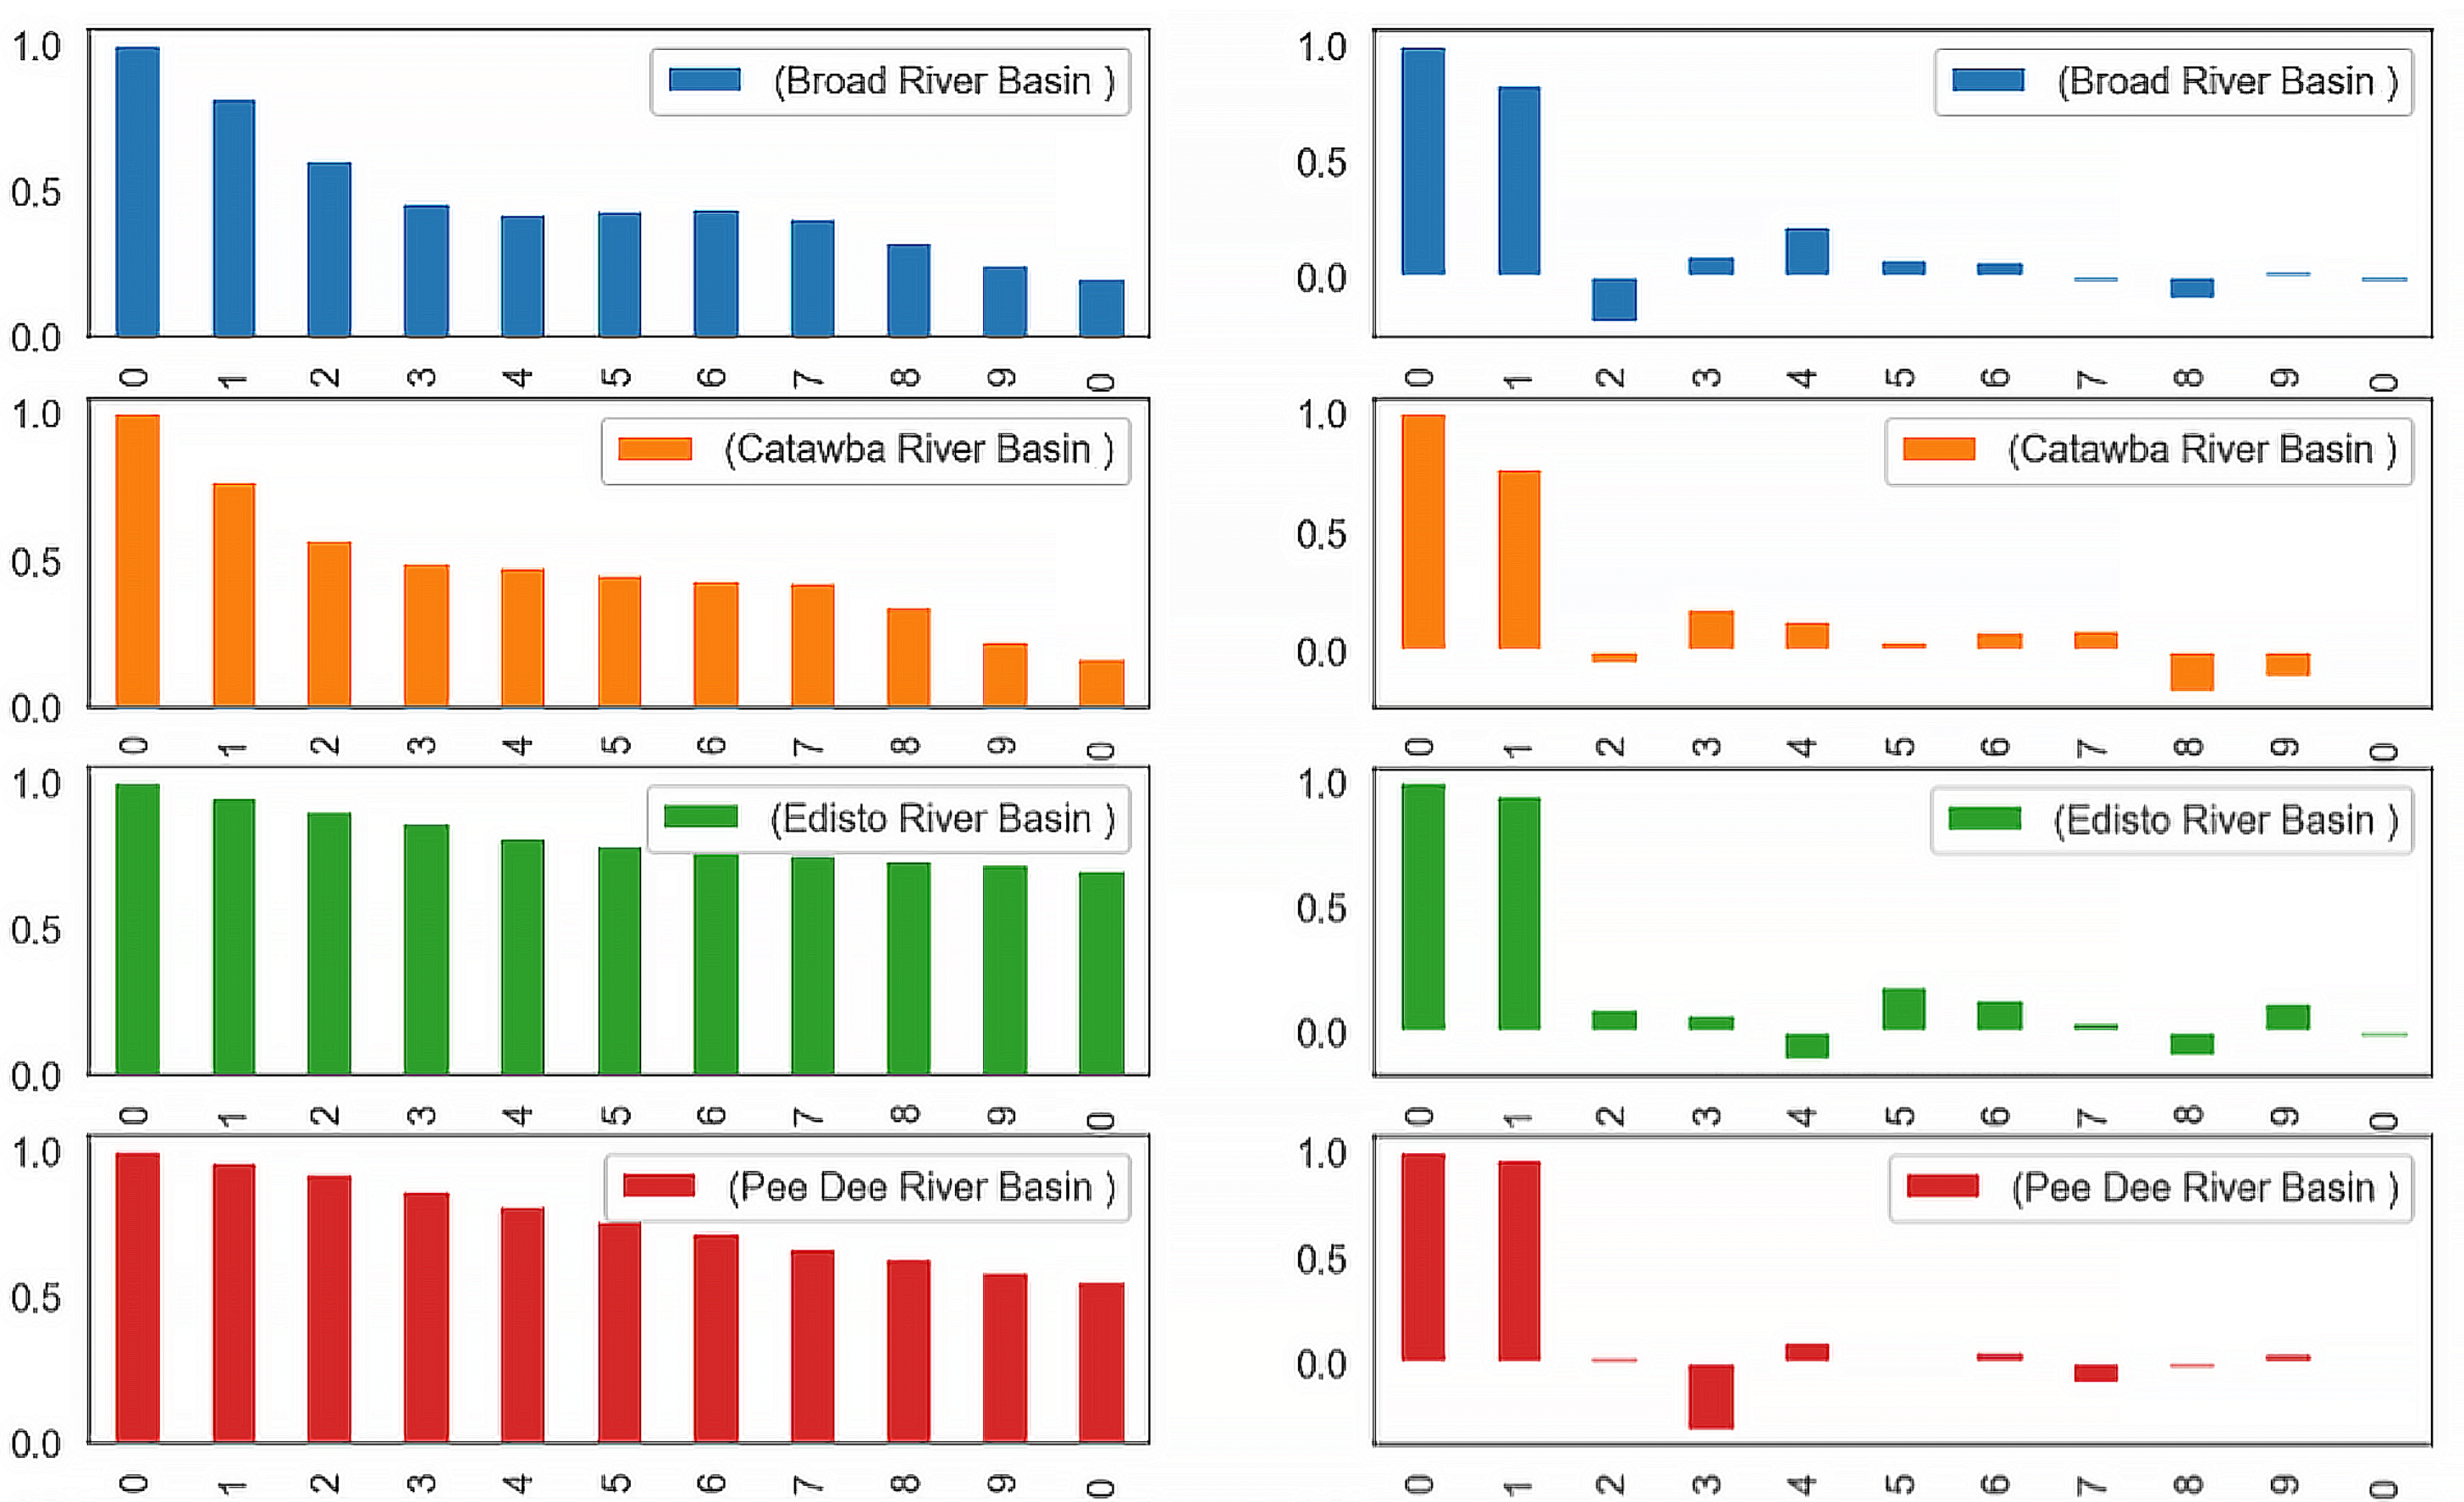
\includegraphics[width=0.8\textwidth]{../images/acf_and_pacf_for_residuals.png}
\caption{\hl{The ACF and PACF of residuals from the CAR model without autoregressive term.}}
\label{fig:ACF_and_PACF}
\end{center}
\end{figure}

To further evaluate the effectiveness of the autoregressive model, we show a time series plot (Figure~\ref{fig:resid_time_series}, left panel) after averaging out residuals spatially.
We also calculate the 2.5\% and 97.5\% percentiles, and thus the shaded area indicates the range of 95\% of all residuals.
 No apparent autocorrelation pattern is detected, although the last few  observations indicate increased volatility in  gage height.
 The absence of an autocorrelation pattern is attributed to the autoregressive term, since a  CAR model without the AR(1) term gives the residual time series plot that shows a more obvious autocorrelation  pattern and more variability (Figure~\ref{fig:resid_time_series}, right panel).\\

\begin{figure}[htbp]
\centering
\includegraphics[width=1\textwidth]{../images/residuals_over_time_for_ar_and_non_ar.png}
\caption{\hl{The time series plot of residuals from the CAR model. The shaded area contains {95\%} of residuals at each time point. Left panel: with AR(1) term. Right panel: without AR(1) term.}}
\label{fig:resid_time_series}
\end{figure}

\hl{In addition, we examine several time series plots at multiple locations in Figure~{\ref{fig:per_site}}.
We picked four stations of varying degrees of volatility for demonstration purpose, each from a different HUC-6 area.
Station 02172002, for example, has rarely seen drastic changes in gage height over the five year between 2012
and 2016.
The only exception is during the 2015 flood event.
In contrast, Station 02197500 demonstrates a different pattern which is more variable and not dominated by the 2015
event.
Overall, the autoregressive model consistently captures the trend across different HUC-6 area locations
with no systematic overestimation or underestimation.
The calculation of mean squared error per site also validates this conclusion.} \\

\begin{figure}[htbp]
\centering
\includegraphics[width=1\textwidth]{../images/prediction_of_four_sites.png}
\caption{\hl{Time series plot of predicted gage height and observed gage height at multiple locations.}}
\label{fig:per_site}
\end{figure}

From a spatial perspective, we examine the distribution of residuals by visualizing them on a map with different colors representing \hl{negative and positive errors} (Figure~\ref{fig:spatial_resid}).
The radius of the circle is proportional to the residual.
This is a daily snapshot on October 3, 2015, from which one can conclude that the residuals are fairly evenly distributed.
Several randomly selected snapshots have been examined during the five-year span and no significant sign of overestimation or underestimation is observed.
 Additionally, one can  aggregate the residuals over a time period, for instance, a year, and make a yearly residual map for inspection.
 Such visualization presents a similar picture as Figure~\ref{fig:spatial_resid} and is thus omitted for the sake of space. \\

\begin{figure}
 \begin{center}
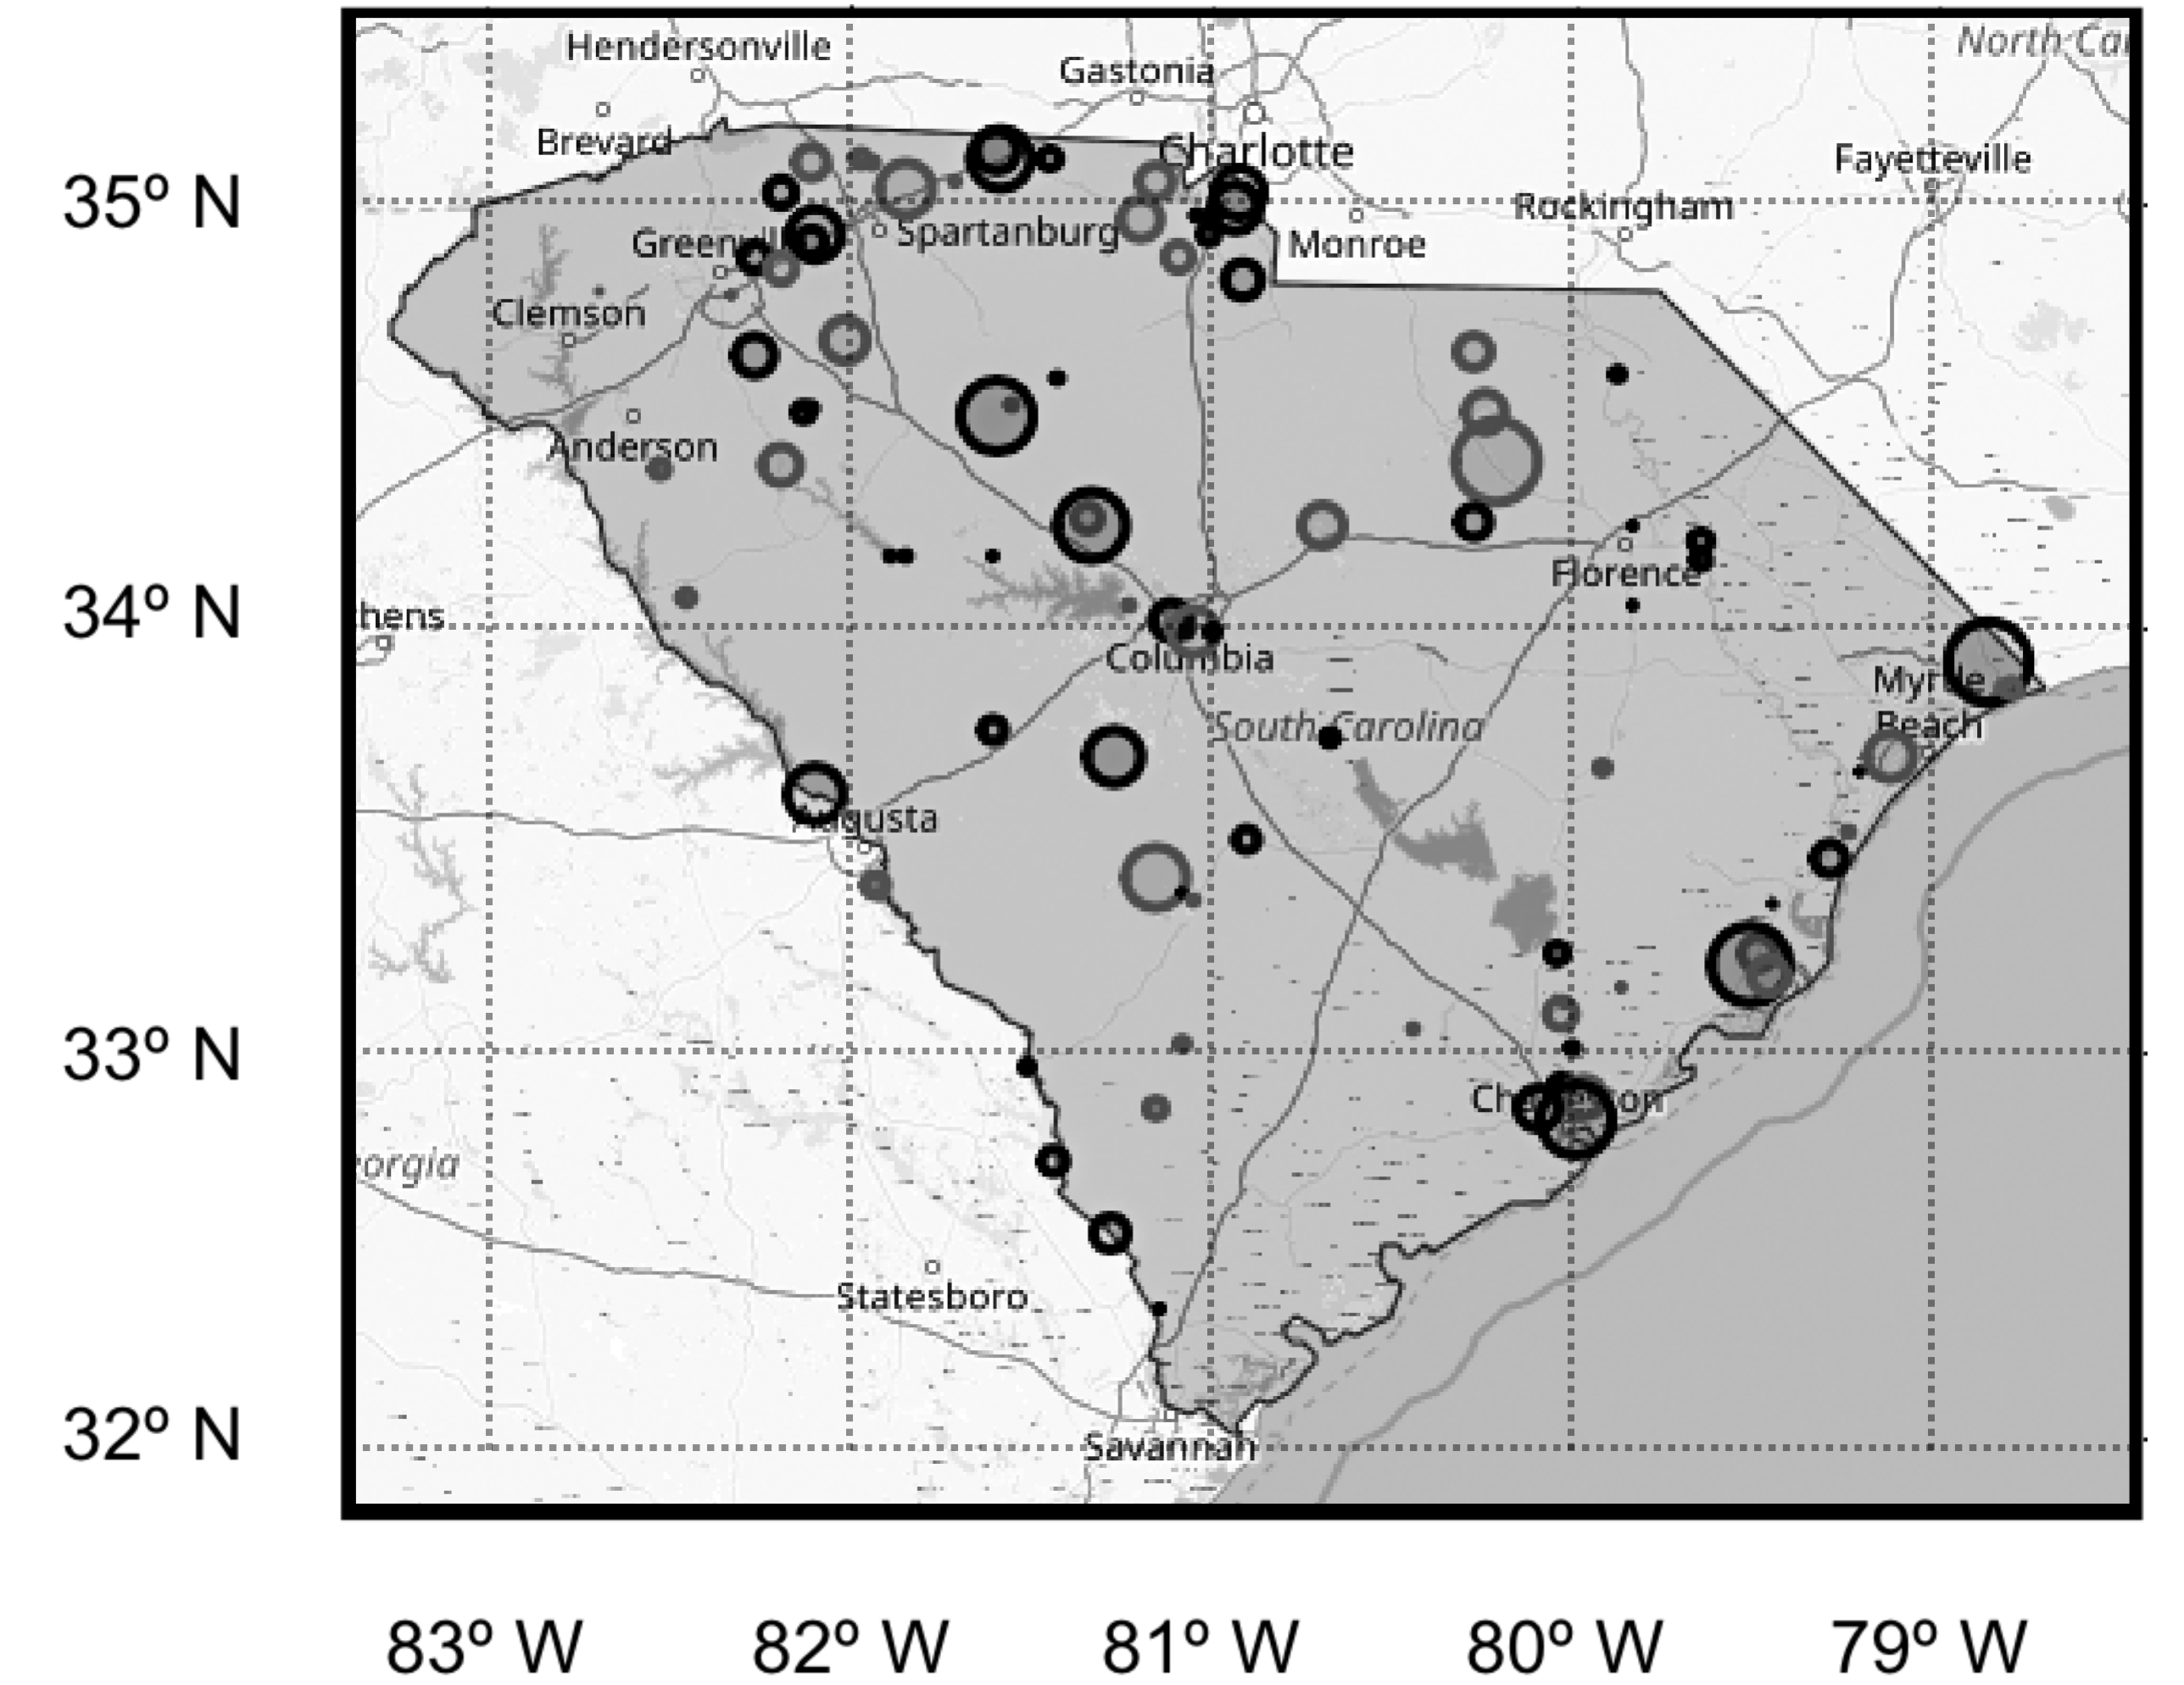
\includegraphics[width=0.6\textwidth]{../images/residuals_on_map.png}
\caption{The residuals from the CAR model on the map of SC. Gray circles indicate negative errors (overestimation) and black circles indicate positive errors (underestimation).}
\label{fig:spatial_resid}
 \end{center}
\end{figure}

Recall that our fitted model presented in Section~\ref{sec:model_fitting} used a non-normal error structure;
We now explain that choice.
If we fit a model with a normal error distribution and \hl{examine the qq (quantile-quantile) plot (Figure}~\ref{fig:hist_original}(b)), we perceive  a pattern that suggests heavy-tailed errors and thus a violation of normality.
This is potentially due to the heavy-tailed distribution of maximum gage heights \hl{(Figure}~\ref{fig:hist_original}(a)).
Note that the observations are plotted after the aforementioned scaling operation.
The data are also slightly skewed to the right possibly due to occasional thunderstorms, which cause short-term, sharp and severe rises in the gage heights.
\hl{Flow dynamics in the eastern US are mainly governed by landfall of tropical cyclones and extratropical systems.
Tail asymmetry can be partly related to the mixed dynamics forcing floods in different seasons (Smith, 2011)}.
Instead of normal errors, using an error structure that follows either a t or Laplace distribution handles extreme rainfall values better.
Specifically, we pick a t distribution with 3 degrees of freedom since $ \nu =3$ defines a distribution with reasonably heavy tails and  guarantees that both expectation and variance exist.
Alternatively, one can also set $\nu$ as a hyper-parameter which can be sampled from the posterior distribution.
\hl{Another possible error distribution could be a skew-t distribution, although for this data set the symmetric heavy-tailed error distributions provide a good fit}. \\

\begin{figure}[htbp]
 \begin{center}
     \includegraphics[width=\textwidth]{../images/qq_and_hist_gage_height_after_scaling.png}
\caption{(a): The histogram of gage heights after scaling. (b): The qq plot residuals assuming normal errors.}
\label{fig:hist_original}
 \end{center}
\end{figure}

The t distribution where $ \nu =3 $ (right panel, Figure~\ref{fig:qq_comp}) is slightly better in terms of its qq plot than the Laplace (left panel, Figure~\ref{fig:qq_comp}).
Hence, the estimation reported in section~\ref{subsec:reported_result} was based on the model assuming that the error term follows a t distribution with 3 degrees of freedom.
Note that the parameter estimates would be similar for the two models assuming either of the heavy-tailed distributions (t or Laplace).

\begin{figure}[htbp]
 \begin{center}
\includegraphics[width=1\textwidth]{../images/qq_plot_for_residuals.png}
\caption{The qq plots of residuals assuming Laplace (left) and t with 3 degrees of freedom (right) distributions.}
\label{fig:qq_comp}
 \end{center}
\end{figure}

\section{Model Comparison}\label{sec:model_comp}
It is of interest to evaluate the forecasting capability of the aforementioned CAR model since the gage observations, in and of themselves, are time series data, and forecasting realtime and future flood events might be helpful for early warning systems and emergency management.
We compare out-of-sample predictions for the first week of 2017 with the ground truth and calculate the mean squared error and the mean absolute error as metrics since such calculations can be applied to any type of models as long as the response variables are continuous.
\hl{Note that the rainfall and gage height data are measured simultaneously, so that the rainfall at a particular time is used to predict or explain the flooding at the same time. We have found that the time lag between the rainfall cause and the flooding consequence is minimal.  However, note that in practice, the use of this model for real-time forecasting of flooding would require some projections of rainfall into the future. The use of the model for retrospective explanatory purposes after the flooding was observed would not require such projections, of course.}

In addition, we consider several other models to compare with the CAR model: specifically, the general linear regression model, and two members of a popular family of classification and regression methods:  random forest and boosting trees.
 Comparing the linear model with CAR highlights the necessity of including a proximity matrix since a customized covariance structure is the major difference.
 Random forest and boosting trees, two popular machine learning algorithms, predict the patterns in data by combining the outputs of individual trees and can give decent benchmarks of model performance.
 Random forest and boosting trees are both tree-based algorithms and entropy is used as the loss function, but the random forest works in parallel while adaptive boosting works sequentially.
 Specifically, a random forest obtains results by taking the average of each decision tree prediction, while adaptive boosting builds decision trees iteratively, and the weight of each observation is adjusted until convergence. \\

\hl{The random forest method (Breiman, 2001) and boosting trees (Friedman, 2001) are chosen as benchmark models since they are routinely used in water sciences.
For example, the random forest regression model is demonstrated to be effective in unsaturated hydraulic conductivity and superior to the M5 tree model (Sihag, 2015).
A random forest approach is also applied in forecasting the spatial distribution of sediment pollution and detecting its predictors (Walsh, 2017).
Tyralis (2019) provided a thorough overview of recent papers which involve the study of hydrology and random forest applications, whose themes include rainfall runoff model, streamflow forecasting and  drought prediction.}\\

For a fair comparison, all three models include the same seven covariates as the CAR model: precipitation, seasonality variables and all related interaction terms.
It is worth noting that the spatial information is handled differently between the CAR model and the other benchmark models.
Rather than defining a covariance matrix based on the basin information, we include the water basin indicator as a  categorical variable.
The mean squared error (MSE) and the mean absolute error (MAE) are reported in Table~\ref{com_model_fit}.
As seen in Table~\ref{com_model_fit}, the CAR model outperforms the benchmark models by a considerable margin.
\hl{In general, the CAR model is better at exploiting the spatial dependency while the random forest algorithm makes better use of covariates.
Therefore the large difference between the two models in MAE and MSE can be explained by the small number of covariates.}
This notion can be \hl{further} substantiated by examining the feature importance of the random forest and boosting trees (feature importance  is  measured by the amount of entropy reduced after a variable is added to the full model), since these two models assign almost negligible importance to the watershed variables (Table~\ref{com_model_fit_trees}).
 On the other hand, consistent with the CAR model, the benchmark models such as the random forest recognize  precipitation as a major contributor to the flood  height (with a feature importance value of 0.6720 based on random forest, 0.4686 based on boosting trees).

\begin{table*}[htbp]
\caption{The comparison of the out-of-sample predictions.}
\centering
\begin{tabular}{|c|l|l|}
\hline
Model &  MAE &   MSE \\ \hline
CAR model & 0.3077 &0.2903  \\ \hline
Linear Model &1.2638 &3.0411 \\ \hline
Random Forest &1.3041 & 3.4282  \\ \hline
Boosting Trees &1.5557 &4.3659 \\ \hline
\end{tabular}
\label{com_model_fit}
\end{table*}

\begin{table*}[htbp]
\caption{A comparison of feature importances for random forest model  and boosting trees.}
\centering
\begin{tabular}{|l|l|l|}
\hline
Watershed &  Random Forest &   Boosting Trees \\ \hline
Santee & 0.0229  & 0.1751\\ \hline
Lower Pee Dee & 0.0327 & 0.0133\\ \hline
Savannah  &0.0439   &0.0245\\ \hline
Edisto SC Coastal  &0.0042 &0.0441 \\ \hline
\end{tabular}
\label{com_model_fit_trees}
\end{table*}

\hl{To validate the conclusion, we also compute the MSE based on leave-one-out (LOO) cross-validation based on locations.
We use LOO rather than traditional K-fold cross-validation to avoid the computational burden of partitioning the data (locations) repeatedly and fitting the model on every partition.
Vehtari et al. (2016) introduced an efficient computation of LOO from MCMC samples,
which uses Pareto-smoothed importance sampling (PSIS) to provide an estimate
of point-wise out-of-sample prediction accuracy.
The CAR model, in this experiment, gives an MSE of 0.32, which outperforms linear model (1.12), random forest (1.32) and boosting
trees (1.66), consistent with outcome of the one-week forecast task.}











\section{Discussion}\label{sec:discussion}

We have presented a spatiotemporal model for gage height in South Carolina from 2011 to 2015, a period including one of the most destructive storms in state history.
Our model accounts for the heavy-tailed pattern of the response variable and allows us to determine several covariates that affect the gage height and to interpret their effects.
In particular, due to the effect of interactions, a stronger association between precipitation and flooding can be observed during summer compared to other times of the year.
If reliable precipitation forecasts are available, our model could be used for forecasting realtime and future flood events, potentially aiding early warning systems and emergency management.\\

In addition, we developed a Python library to streamline the data preprocessing steps.
Data scraping,  cleaning, aggregating and transforming steps can be done by simple function calls.
We demonstrate several reusable modules we have developed  by providing some basic examples in the Github repository of our package.
Our hope is that such tools will enable straightforward employment of similar spatio-temporal models for flood data in the future.


\appendix
\section{Appendix}\label{sec:appendix}
\nonumber
\subsection{Sparse Matrix}\label{subsec:sparse}

A \emph{sparse} matrix is a matrix where most elements are zero.
By contrast, a matrix is considered \emph{dense} if most elements are nonzero.
A measure to quantify the sparsity of a matrix is the number of zero-valued elements divided by the total number of elements.
As a rule of thumb, a matrix is considered sparse when its sparsity is greater than 0.5. The covariance matrix in the aforementioned CAR model is largely based on our adjacency model, and has a sparsity of 0.86.\\

Once a sparse matrix is recognized, one can use specialized algorithms and data structures to accelerate computation.
This is because memory and computing power are wasted on the zeroes if we employ a standard dense-matrix algorithm.
Specifically, a dense matrix is typically stored as a two-dimensional array, and each entry in the array represents an element $ a_{ij}$ of the matrix.
One can access any element by specifying the row index $i$ and the column index $j$.
In contrast, in a typically sparse matrix representation, only the nonzero entries are stored and thus memory use can be reduced substantially.
As a tradeoff, retrieving individual elements becomes more complex in a sparse matrix.\\

In practice, there are several representations of a sparse matrix.
While some types stand out for their efficient modification, such as DOK (Dictionary of Keys) and COO (Coordinate List), others, e.g., Compressed Sparse Row (CSR), support fast matrix operations.
CSR suits our needs better since evaluating a multivariate normal distribution involves matrix multiplication, and thus is implemented as part of our model. \\

The compressed sparse row (CSR) represents a matrix by three one-dimensional arrays: the nonzero values, the row indices, and the column indices.
Note that the row indices are not defined in a straightforward manner.
An example is given as follows to demonstrate how a CSR representation is implemented.

\begin{align*}
\left(
\begin{matrix}
  0 & 0 & 0 & 0 \\
  5 & 8 & 0 & 0 \\
  0 & 0 & 3 & 0 \\
  0 & 1 & 0 & 0
\end{matrix}
\right)
\end{align*}

\noindent The three vectors to represent the example sparse matrix is
\begin{verbatim}
A  = [5, 8, 3, 6]   IA = [0, 0, 2, 3, 4]   JA = [0, 1, 2, 1].
\end{verbatim}

The array \texttt{A} is the nonzero values, whose column indices are stored in  \texttt{JA}.
For instance, 3 is in the third column and thus the third element in \texttt{JA}  is 2, which stands for the third column since a zero-based index is used.
On the other hand, \texttt{IA}  contains the row information and is defined recursively, where  \texttt{IA[0] = 0}  and  \texttt{IA[i] = IA[i-1] + k}.
Note that \texttt{k} is  number of nonzero elements on the $i$th row in the original matrix.
According to this definition, the length of \texttt{IA} is $m + 1$ when the matrix has $ m $ columns, and the last element in \texttt{IA} is always the number of nonzero values.\\

The sparse matrix stored in CSR is efficient in matrix-vector multiplication due to the structure of \texttt{IA} and \texttt{JA}.
For instance, multiplying \texttt{[5, 8, 0,0]} by another vector, say \texttt{[1, 0, 9, 9]}, requires only retrieving nonzero values at location 0 and 1 from the second row.
The location information is conveniently stored in \texttt{JA}, and the length of nonzero values can be found in \texttt{IA}.
 Since we only need to compute the dot product of \texttt{[5, 8]} and \texttt{[1, 0]}, the computation is reduced by half.
  In practice, we observe a six-to-ten times boost in sampler performance by switching from a dense matrix implementation, since the adjacency matrix has greater sparsity.


\begin{thebibliography}{9}
\bibitem{7}
Banerjee, S., Carlin, B. P.,  Gelfand, A.\ E.\ (2014).\ Hierarchical modeling and analysis for spatial data.
CRC Press, Boca Raton.

\bibitem{runoff}
Betson, R. P.\ (1964).\ What is watershed runoff?
Journal of Geophysical Research, 69(8):1541-1552.

\bibitem{bonnin}
Bonnin, G. M., Martin, D., Lin, B., Parzybok, T., Yekta, M., \& Riley, D.\ (2006).\
Precipitation-frequency atlas of the United States.
NOAA atlas, 14(2): 1--65.

\bibitem{random-forest}
\hl{Breiman} L.\ (2001).\ Random forests.
Machine Learning 45(1): 5--32.
\url{https://doi.org/10.1023/A:1010933404324}

\bibitem{clark}
Clark MP et al.\ (2015).\ A unified approach for process-based hydrologic modeling:
1.\ Modeling concept.
Water Resource Research 51: 2498--2514. \url{https://doi.org/10.1002/2015WR017198}

\bibitem{new11}
Ciach, G. J.,  Krajewski, W. F.\ (2006).\ Analysis and modeling of spatial correlation structure in small-scale rainfall in central Oklahoma.
Advances in Water Resources, 29(10), 1450--1463.

\bibitem{2}
Cressie, N. (1993).\ Statistics for spatial data.
John Wiley \& Sons, New York.

\bibitem{flood2}
Daly, C., Neilson, R. P.,  Phillips, D. L.\ (1994).\ A statistical-topographic model for mapping climatological precipitation over mountainous terrain.
Journal of Applied Meteorology, 33(2): 140--158.

\bibitem{flood1}
Daly, C., Taylor, G. H., Gibson, W. P., Parzybok, T. W., Johnson, G. L., Pasteris, P. A.\ (2000).\
High-quality spatial climate data sets for the United States and beyond.
Transactions of the ASAE, 43(6): 1957.

\bibitem{new14}
Deidda, R.\ (2000).\ Rainfall downscaling in a space-time multifractal framework.
Water Resources Research, 36(7): 1779--1794

\bibitem{new23}
Delhomme, J. P.\ (1978).\ Kriging in the hydrosciences.
Advances in Water Resources, 1(5): 251--266.

\bibitem{new22?}
Delfiner, P., Delhomme, J. P.\ (1975).\ Optimum interpolation by kriging.
Ecole Nationale Sup{\'e}rieure des Mines, Paris.

\bibitem{new9}
Diggle, P. J., Tawn, J. A., Moyeed, R. A.\ (1998).\  Model-based geostatistics.
Journal of the Royal Statistical Society: Series C (Applied Statistics), 47(3): 2299--350

\bibitem{new26}
Dumitrescu, A., Birsan, M. V., Manea, A.\ (2016).\ Spatio-temporal interpolation of sub-daily (6 h) precipitation over Romania for the period 1975--2010.
International Journal of Climatology, 36(3): 1331--1343.

\bibitem{strm}
Farr, T. G., Rosen, P. A., Caro, E., Crippen, R., Duren, R., Hensley,  Kobrick, M. et al.\ (2007).\ The shuttle radar topography mission.
Reviews of Geophysics, 45(2).

\bibitem{new12}
Ferraris, L., Gabellani, S., Rebora, N.,  Provenzale, A.\ (2003).\
A comparison of stochastic models for spatial rainfall downscaling.
Water Resources Research, 39(12).

\bibitem{fred}
Frederick, R.H.\ and Miller, J.F.\ (1979).\ Short duration rainfall frequency relations for California.
Third Conference on Hydrometeorology, Bogata, Columbia.
American Meteorological Society, 667--73

\bibitem{greedy_function}
\hl{Friedman}, J. H.\ (2001).\ Greedy function approximation: A gradient boosting machine.
The Annals of Statistics 29(5): 1189--1232. \url{https://doi.org/10.1214/aos/1013203451}

\bibitem{new15}
Georgakakos, K. P., Kavvas, M. L.\ (1987).\ Precipitation analysis, modeling, and prediction in hydrology.
Reviews of Geophysics 25(2): 163--178.

\bibitem{new8}
Hastings, W. K.\ (1970).\ Monte Carlo sampling methods using Markov chains and their applications.
Biometrika, 57(1): 97--109.

\bibitem{koutsoyiannis2}
Koutsoyiannis D.\ (2011).\ Hurst-Kolmogorov dynamics and uncertainty.
J Am Water Resour Assoc, 47(3): 481--95.
\url{http://dx.doi.org/10.1111/j.1752- 1688.2011.00543.x.}

\bibitem{koutsoyiannis3}
Koutsoyiannis D, Montanari A.\ (2014).\ Negligent killing of scientific concepts: the stationarity case.
Hydrol Sci J. \url{http://dx.doi.org/10.1080/ 02626667.2014.959959.}

\bibitem{new13}
Kumar, P., Foufoula-Georgiou, E.\ (1994).\ Characterizing multiscale variability of zero intermittency in spatial rainfall.
Journal of Applied Meteorology, 33(12): 1516--1525.

\bibitem{new25}
Ly, S., Charles, C., Degre, A.\ (2011).\ Geostatistical interpolation of daily rainfall at catchment scale:
The use of several variogram models in the Ourthe and Ambleve catchments, Belgium.
Hydrology and Earth System Sciences, 15(7): 2259--2274.

\bibitem{14}
Matheron, G.\ (1963).\ Principles of geostatistics.
Economic geology, 58(8): 1246--1266.

\bibitem{new17}
Isaaks, H.\ E., Srivastava, R.\ M.\ (1989).\ Applied geostatistics.
Oxford University Press, New York.

\bibitem{new7}
Metropolis, N., Rosenbluth, A. W., Rosenbluth, M. N., Teller, A. H., Teller, E.\ (1953).\
Equation of state calculations by fast computing machines.
The Journal of Chemical Physics, 21(6):1087-1092.

\bibitem{10}
National Oceanic and Atmosphere Administration, U.S.\ Department of Commerce.\ (2015).\
Service assessment: The historic South Carolina floods of October 1--5, 2015.
Accessed at \path{www.weather.gov/media/publications/assessments/SCFlooding_072216_Signed_Final.pdf} on December 4, 2017.

\bibitem{phillips}
Phillips, R. C., Samadi, S., Meadows, M.E.\ (2018).\ How extreme was the October 2015 flood in the Carolinas?
An assessment of flood frequency analysis and distribution tails.
Journal of Hydrology, DOI: https://doi.org/10.1016/j.jhydrol.2018.05.035

\bibitem{samadi2}
Samadi S., Tufford D., Carbone, G.\ (2018).\
Estimating hydrologic model uncertainty in the presence of complex residual error structures.
Stochastic Environmental Research and Risk Assessment, 32(5): 1259--1281. \url{DOI: 10.1007/s00477-017-1489-6.}

\bibitem{samadi}
Samadi, S. Z.,  M. E. Meadows.\ (2017).\
The transferability of terrestrial water balance components under uncertainty and nonstationarity:
A case study of the coastal plain watershed in the southeastern USA\@.
River research and applications, 33, no.\ 5:796-808.

\bibitem{reviewer2}
Serinaldi, F., Kilsby, C.G.\ (2014).\
Rainfall extremes: Toward reconciliation after the battle of distributions.
Water Resources Research, 50: 336--352.

\bibitem{seaber}
Serinaldi, F.,  Kilsby C. G.\ (2015).\
Stationarity is undead: Uncertainty dominates the distribution of extremes.
Adv.\ Water Resour 77: 17--36, \url{doi:10.1016/j.advwatres.2014.12.013.}

\bibitem{huc}
Seaber, P.\ R., Kapinos, F.\ P.,  Knapp, G. L.\ (1987).\ Hydrologic unit maps.
Accessed at \url{https://pubs.usgs.gov/wsp/wsp2294/html/pdf.html}

\bibitem{new24}
Sharon, D.\ (1972).\ Spatial analysis of rainfall data from dense networks.
 Hydrological Sciences Journal 17(3): 291--300.

\bibitem{randomforest_usage}
Sihag, P., Mohsenzadeh S.,  Angelaki, A.\ (2019).\ Random forest, M5P and regression analysis to estimate the field unsaturated hydraulic conductivity.
Applied Water Science, 9(5): 129.
\url{https://doi.org/10.1007/s13201-019-1007-8}

\bibitem{distribution_1}
Smith, J.\ A., Villarini G., Baeck, M.\ L.\ (2011).\ Mixture Distributions and the Hydroclimatology of Extreme Rainfall and Flooding in the Eastern United States.
Journal of Hydrometeorology, 12, 294--309.
\url{https://doi.org/10.1175/2010JHM1242.1.}

\bibitem{new20}
Thiessen, A.\ H.\ (1911).\ Precipitation averages for large areas.
Monthly Weather Review, 39(7): 1082--1084.

\bibitem{randomforest_usage_3}
Tyralis, H., Papacharalampous, G., Langousis, A.\ (2019).\
A brief review of random forests for water scientists and practitioners and their recent history in water resources.
Water, 11(5): 910.

\bibitem{loo_waic}
Vehtari, A., Gelman, A.,  Gabry, J.\ (2017).\
Practical Bayesian model evaluation using leave-one-out cross-validation and WAIC\@.
Statistics and Computing, 27(5): 1413--1432.

\bibitem{reviewer}
Villarini, G.\ et al.\ (2009) .\ Flood frequency analysis for nonstationary annual peak records in an urban drainage basin.
Advances in Water Resources 32: 1255--1266.

\bibitem{randomforest_usage_2}
Walsh, E.S., Kreakie, B.J., Cantwell, M.G.,  Nacci, D.\ (2017).\
A Random Forest approach to predict the spatial distribution of sediment pollution in an estuarine system.
PloS one, 12(7): e0179473.

\bibitem{ggplot}
Wickham, Hadley.\ (2016).\ ggplot2: Elegant graphics for data analysis.
New York, Springer.

\end{thebibliography}
\end{document}

